\documentclass[10pt]{article}
\usepackage[utf8]{inputenc}
\usepackage[T1]{fontenc}
\usepackage{amsmath}
\usepackage{amsfonts}
\usepackage{amssymb}
\usepackage{mhchem}
\usepackage{stmaryrd}
\usepackage{graphicx}
\usepackage[export]{adjustbox}
\graphicspath{ {./images/} }
\usepackage{bbold}

\begin{document}
\section{Contents}
1 Polynomials, Finite Element and Neural Network Functions $\ldots \ldots \ldots$. 5

1.1 Approximation by polynomials and Weierstrass Theorem $\ldots \ldots \ldots .5$

1.1.1 Weierstrass Theorem and Proof $\ldots \ldots . . . . . . . . . . . . . .$

1.1.2 Some issues with polynomial approximations $\ldots \ldots \ldots . . .7$


\includegraphics[max width=\textwidth]{2022_01_05_fba364634dde0bb701e1g-2}

\section{Polynomials, Finite Element and Neural Network}
In this chapter, we discuss approximation properties of spaces of polynomials and finite elements consisting of piecewise polynomials.

\subsection{Approximation by polynomials and Weierstrass Theorem}
Let $\alpha=\left(\alpha_{1}, \cdots, \alpha_{d}\right)$ with $\alpha_{i}$ being non-negative integers, we note $|\alpha|=\sum_{i=1}^{d} \alpha_{i}$ and
$$
x^{\alpha}=x_{1}^{\alpha_{1}} x_{2}^{\alpha_{2}} \cdots x_{d}^{\alpha_{d}} .
$$
We use $\mathbb{P}_{m}\left(\mathbb{R}^{d}\right)$ to define the polynomials of $d$-variables of degree less than $m$ which consists functions of the form
$$
\sum_{|\alpha| \leq m} a_{\alpha} x^{\alpha}=\sum_{\alpha_{1}+\alpha_{2}+\ldots+\alpha_{d} \leq m} a_{\alpha_{1}, \ldots, \alpha_{d}} x_{1}^{\alpha_{1}} x_{2}^{\alpha_{2}} \cdots x_{d}^{\alpha_{d}}
$$

\subsubsection{Weierstrass Theorem and Proof}
Important property: polynomials can approximate any reasonable function!

  \begin{itemize}
    \item dense in $C(\Omega)$ [Weierstrass theorem]

    \item dense in all Sobolev spaces: $L^{2}(\Omega), W^{m, p}(\Omega), \ldots$

  \end{itemize}
Theorem 1. Let $\Omega \subset R^{n}$ be a closed and bounded set. Given any continuous function $f(x)$ on $\Omega$, there exists a sequence of polynomials $\left\{P_{n}(x)\right\}$ such that
$$
\lim _{n \rightarrow \infty} \max _{x \in \Omega}\left|f(x)-P_{n}(x)\right|=0
$$
Proof. Let us first give the proof for $d=1$ and $\Omega=[0,1] .$ Given $f:[0,1] \rightarrow R$ be a continuous function.

Let
$$
\tilde{f}(x)=f(x)-l(x)
$$
where $l(x)=f(0)+x(f(1)-f(0))$. Then $\tilde{f}(0)=\tilde{f}(1)=0$. Noting that $l(x)$ is a linear function, hence without lose of generality, we can only consider the case $f:[0,1] \rightarrow R$ with $f(0)=f(1)=0$

Since $f$ is continuous on the closed interval $[0,1]$, then $f$ is uniformly continuous on $[0,1]$.

First we extend $f$ to be zero outside of $[0,1]$ and obtain $f: R \rightarrow R$, then it is obviously that $f$ is still uniformly continuous.

Next for $0 \leq x \leq 1$, we construct
$$
p_{n}(x)=\int_{-1}^{1} f(x+t) Q_{n}(t) d t=\int_{-x}^{1-x} f(x+t) Q_{n}(t) d t=\int_{0}^{1} f(t) Q_{n}(t-x) d t
$$
where $Q_{n}(x)=c_{n}\left(1-x^{2}\right)^{n}$ and
$$
\int_{-1}^{1} Q_{n}(x) d x=1
$$
Thus $\left\{p_{n}(x)\right\}$ is a sequence of polynomials.

Since
$$
\begin{aligned}
\int_{-1}^{1}\left(1-x^{2}\right)^{n} d x &=2 \int_{0}^{1}\left(1-x^{2}\right)^{n} d x=2 \int_{0}^{1}(1-x)^{n}(1+x)^{n} d x \\
& \geq 2 \int_{0}^{1}(1-x)^{n} d x=\frac{2}{n+1}>\frac{1}{n}
\end{aligned}
$$
Combing with $\int_{-1}^{1} Q_{n}(x) d x=1$, we obtain $c_{n}<n$ implying that for any $\delta>0$
$$
0 \leq Q_{n}(x) \leq n\left(1-\delta^{2}\right)^{n} \quad(\delta \leq|x| \leq 1)
$$
so that $Q_{n} \rightarrow 0$ uniformly in $\delta \leq|x| \leq 1$ as $n \rightarrow \infty$.

Given any $\epsilon>0$, since $f$ in uniformly continuous, there exists $\delta>0$ such that for any $|y-x|<\delta$, we have
$$
|f(y)-f(x)|<\frac{\epsilon}{2}
$$
Finally, let $M=\max |f(x)|$, using $(1.8),(1.4)$ and $(1.7)$, we have
$$
\begin{aligned}
\left|p_{n}(x)-f(x)\right| &=\left|\int_{-1}^{1}(f(x+t)-f(t)) Q_{n}(t) d t\right| \leq \int_{-1}^{1}|f(x+t)-f(t)| Q_{n}(t) d t \\
& \leq 2 M \int_{-1}^{-\delta} Q_{n}(t) d t+\frac{\epsilon}{2} \int_{-\delta}^{\delta} Q_{n}(t) d t+2 M \int_{\delta}^{1} Q_{n}(t) d t \\
& \leq 4 M n\left(1-\delta^{2}\right)^{n}+\frac{\epsilon}{2}<\epsilon
\end{aligned}
$$
for all large enough $n$, which proves the theorem.

The above proof generalize the high dimensional case easily. We consider the case that
$$
\Omega=[0,1]^{d} .
$$
By extension and using cut off function, W.L.O.G. that we assume that $f=0$ on the boundary of $\Omega$ and we then extending this function to be zero outside of $\Omega$.

Let us consider the special polynomial functions
$$
Q_{n}(x)=c_{n} \prod_{k=1}^{d}\left(1-x_{k}^{2}\right)
$$
Similar proof can then be applied. $\square$

\subsubsection{Some issues with polynomial approximations}
\section{Curse of dimensionality}
Number of coefficients for polynomials of degrees $n$ in $\mathbb{R}^{d}$ is
$$
N=\left(\begin{array}{c}
d+n \\
n
\end{array}\right)=\frac{(n+d) !}{d ! n !}
$$
For example $n=100$ :

\begin{tabular}{|c|c|c|c|}
\hline
$d=$ & 2 & 4 & 8 \\
\hline
$N=$ & $5 \times 10^{3}$ & $4.6 \times 10^{6}$ & $3.5 \times 10^{11}$ \\
\hline
\end{tabular}

\section{Runge's phenomenon}
Consider the case where one desires to interpolate through $n+1$ equispaced points of a function $f(x)$ using the n-degree polynomial $P_{n}(x)$ that passes through those points. Naturally, one might expect from Weierstrass' theorem that using more points would lead to a more accurate reconstruction of $f(x)$. However, this particular set of polynomial functions $P_{n}(x)$ is not guaranteed to have the property of uniform convergence; the theorem only states that a set of polynomial functions exists, without providing a general method of finding one.

The $P_{n}(x)$ produced in this manner may in fact diverge away from $f(x)$ as $\mathrm{n}$ increases; this typically occurs in an oscillating pattern that magnifies near the ends of the interpolation points. This phenomenon is attributed to Runge.

Problem: Consider the Runge function
$$
f(x)=\frac{1}{1+25 x^{2}}
$$
(a scaled version of the Witch of Agnesi). Runge found that if this function is interpolated at equidistant points $x_{i}$ between $-1$ and 1 such that:
$$
x_{i}=\frac{2 i}{n}-1, \quad i \in\{0,1, \ldots, n\}
$$
with a polynomial $P_{n}(x)$ of degree $\leq n$, the resulting interpolation oscillates toward the ends of the interval, i.e. close to $-1$ and 1. It can even be proven that the interpolation error increases (without bound) when the degree of the polynomial is increased:
$$
\lim _{n \rightarrow \infty}\left(\max _{-1 \leq x \leq 1}\left|f(x)-P_{n}(x)\right|\right)=+\infty
$$
This shows that high-degree polynomial interpolation at equidistant points can be troublesome

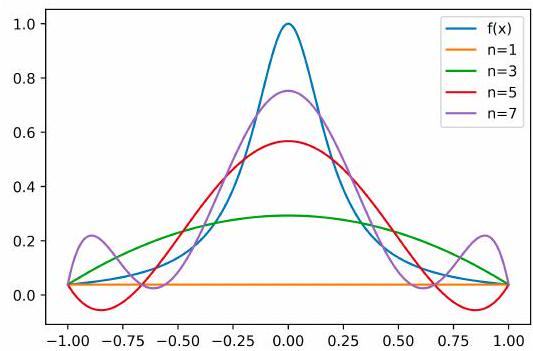
\includegraphics[max width=\textwidth]{2022_01_05_fba364634dde0bb701e1g-6}

Fig. 1.1. Runge's phenomenon: Runge function $f(x)=\frac{1}{1+25 x^{2}}$ and its polynomial interpolation $P_{n}(x)$.


\end{document}